% ====================
% ===================================================
\chapter{Literature}
% ===================================================
% ====================



% ====================
\section{Online RGB Trackers (timeline/history)}
% ====================

\textbf{Tracking-by-detection}

Hare \etal~\cite{hare2014struck}:

\blockquote{An approach to tracking which has become particularly
popular recently is tracking-by-detection \cite{avidan2004support}, which treats
the tracking problem as a detection task applied over time}

Hare \etal~\cite{hare2014struck}:
\blockquote{State-of-the-art adaptive tracking-by-detection methods mainly
focus on improving tracking performance by increasing
the robustness of the classifier to poorly labelled samples
resulting from this approach. Examples of this include using
robust loss functions [6], [7], semi-supervised learning [8],
[9], or multiple-instance learning [3], [10].} 


"The core component of most modern trackers is a discriminative classifier, tasked with distinguishing between the target
and the surrounding environment." \cite{henriques2015tracking}.

"ARGUABLY one of the biggest breakthroughs in recent
visual tracking research was the widespread adoption
of discriminative learning methods" \cite{henriques2015tracking}

\begin{figure}
   \hspace{-2mm}
   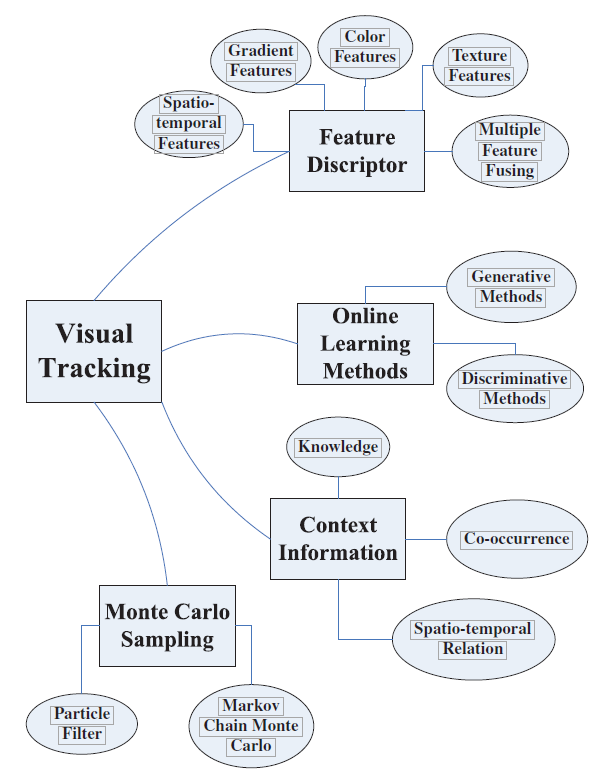
\includegraphics[width=0.45\linewidth]{figures/yang2011recent_graph.png}
   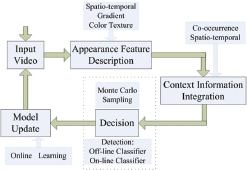
\includegraphics[width=0.45\linewidth]{figures/yang2011recent_flowchart.png}
   \caption{\textbf{Framework of tracking models}. From \cite{avidan2004support}.}
   \label{fig:yang2011recent}
\end{figure}




% ====================
\section{Online RGB Trackers (vision papers)}
% ====================
Survey papers:
\begin{enumerate}
\item Yang et al. \cite{yang2011recent}. 2011 survey of the field
\item \textbf{Pang et al's Survey} \cite{pang2013finding} notes biases in
comparisons: usually new papers list their method as the best (because of a
specific methodology); however second best paper rankings are fairly robust. A
meta-analysis concludes the following methods are competitive: Struck, MIL, TLD,
VTD. 
\item \textbf{an extensive PAMI Survey} \cite{smeulders2013visual} claims Struck
is the best, and analyses specific failure cases and how it affects specific
method
\item \textbf{Appearance Model Survey} \cite{li2013survey}
\item A comprehensive list of papers can be found by searching papers that have
referenced Struck; which is the most frequently used benchmark to compare
against.
\item \textbf{Visual Tracking Benchmark}\cite{kristan2013visual} 
\item Wu et. al \cite{wu2013online} (SCM, Struck, TLD, ASLA, CXT, VTD, VTS, CSK)
concludes
    \begin{enumerate}
    \item \textbf{Background Information}  background
    information is critical for effective tracking. It can be ex-
    ploited by using advanced learning techniques to encode
    the background information in the discriminative model im-
    plicitly (e.g., Struck), or serving as the tracking contex-
    t explicitly (e.g., CXT)
    \item \textbf{local models}  are important for tracking as shown in the performance improvement of local sparse representation (e.g., ASLA and SCM) com-
    pared with the holistic sparse representation (e.g., MTT and
    L1APG). They are particularly useful when the appearance
    of target is partially changed, such as partial occlusion or
    deformation.
    \item \textbf{local models} motion model or dynamic model is cru-
    cial for object tracking, especially when the motion of target
    is large or abrupt. However, most of our evaluated tracker-
    s do not focus on this component. Good location predic-
    tion based on the dynamic model could reduce the search
    range and thus improve the tracking efficiency and robust-
    ness.
    \end{enumerate}
\item VOT2014 Results \cite{kristan2014visual}
\end{enumerate}

``The challenge considers single-camera, single-target, model-free, causal trackers, applied to short-term tracking. The model-free property means that the only supervised training example is provided by the bounding box in the first frame.  The short-term tracking means that the tracker does not perform re-detection after the target is lost. Drifting off the target is considered a failure. The causality means that the tracker does not use any future frames, or frames prior to re-initialization, to infer the object position in the current frame." \cite{kristan2014visual}

``In this paper, we focus on the problem of model-free online tracking of an object,
given only the object’s initial position and previous observations, within a tracking-bydetection
framework."\cite{zhang2014meem}

``Model drift occurs because factors like tracking failure, occlusions and misalignment
of training samples can lead to bad model updates. One remedy is to incorporate the first
frame template or prior knowledge in the online model update procedure [20,15]. However,
relying on a fixed model prior tends to restrict the tracker’s ability to handle large
object appearance changes. Other trackers [22,32,14] use a “censorship mechanism”
where an update is prevented when certain criteria are met (or not met). The detection
of good or bad updates usually relies upon smoothness assumptions for motion and
appearance changes, which are often violated in challenging scenarios. And once the
censorship mechanism fails, these trackers will either miss the chance to evolve or get
trapped in a background region, due to the fact that the model can only evolve forward,
without a mechanism to correct for past mistakes."\cite{zhang2014meem}

% --------------------
\subsection{Pre-CVPR 2013 Trackers}
% --------------------


\paragraph{Online RGB Trackers} require no prior knowledge of the object, and only a bounding box of the target on the original frame. 
A survey of tracking methods \cite{wu2013online} (SCM, Struck, TLD, ASLA, CXT, VTD, VTS, CSK), as well as papers following the survey \cite{supancic2013self}, show the following methods are competitive for this problem:
\begin{enumerate}
\item \textbf{Struck} \cite{hare2011struck}  uses a kernelized structured output SVM to directly learn displacement vectors. Gaussian kernel on 192 haar-like features. Struck's TPAMI paper \cite{hare2014struck}. 

Kernelization does most of the work, but structured SVM formulation avoids arbitrary hand-tuned parameters: "a large part of the performance gains... can be attributed to our use of a kernelised SVM rather than a boosting-based classifier."

``(previous) algorithms separate the adaptation phase of
the tracker into two distinct parts: (i) the generation and
labelling of samples; and (ii) the updating of the classifier."

``we make use of the structured output SVM
framework of Tsochantaridis et al. [15]. In particular, we
extend the online structured output SVM learning method
proposed by Bordes et al. [16], [17] and adapt it to the task
of adaptive object tracking."

\item \textbf{SCM} \cite{zhong2012robust} 
\item \textbf{TLD} \cite{kalal2012tracking} "We develop a novel learning method (P-N learning) which estimates the
errors by a pair of “experts”: (i) P-expert estimates missed detections, and (ii) N-expert estimates false alarms. The learning process is
modeled as a discrete dynamical system and the conditions under which the learning guarantees improvement are found. We describe
our real-time implementation of the TLD framework and the P-N learning.

\item \textbf{APG-L1} \cite{bao2012real} "l1 norm related minimization model".
\item \textbf{MIL} \cite{babenko2009visual} Older well-known tracker using multiple instance learning.
\item \textbf{CXT} \cite{dinh2011context} uses background context
\item \textbf{ASLA} \cite{jia2012visual} 
\item \textbf{Circulant} \cite{henriques2012exploiting} (TPAMI \cite{henriques2015tracking}) uses fourier transformed graham matrix to improve .

The fastest tracker in \cite{wu2013online}.

``a notable optimization
is to use a fast but inaccurate classifier to select promising
patches, and only apply the full, slower classifier on those
[18], [19]."

 


\item Zhang \cite{zhang2012real} "propose a projection to a fixed
random basis, to train a Naive Bayes classifier, inspired
by compressive sensing techniques."
\end{enumerate}


% --------------------
\subsection{Post-CVPR 2013 Trackers}
% --------------------
After Wu et. al's  survey \cite{wu2013online}, the following notable methods were also published:

\begin{enumerate}
\item \textbf{Self-paced learning} \cite{supancic2013self} "we show that an accurate appearance model is considerably more effective than a strong motion model". 
\item \textbf{MEEM} \cite{zhang2014meem} claims state-of-the-art over Struck, SCM, MIL.
\item \textbf{Xiang} \cite{xiang2014monocular}
\item \textbf{Occlusion and motion reasoning for long-term tracking} \cite{hua2014occlusion} "Struck fails in
the presence of long-term occlusions as well as severe viewpoint changes
of the object. In this paper we propose a principled way to combine occlusion and motion reasoning with a tracking-by-detection approach."
\item Color tracker \cite{danelljan2014adaptive} - the \textbf{best}.
\end{enumerate}

% --------------------
\subsection{Analysis}
% --------------------
Struck is a major paper, topping the benchmarks of Pang \cite{pang2013finding}, Wu \cite{wu2013online} and Smeulders \cite{smeulders2013visual}. Notably, newer papers aren't as well-tested and perhaps better. Struck is basically kernelized structured output SVMs, where $(x,y)$ are image patches and displacements. Most of the gains come from the kernelization, though.

Circulant trackers are really, quite good.



% =============================================
\section{Online RGB-D Trackers (vision papers)}
\label{sec:online}
% =============================================
\paragraph{Online RGB-D Trackers} no prior knowledge of the object.
Song et. al's survey \cite{song2013tracking}, show \textbf{incorporating depth into tracking beats the state of the art.} It shows \textbf{Struck} \cite{hare2011struck} and VTD are competitive.

\textbf{Gaussian Process Regression} \cite{gao2014transfer} beats struck and Song et. al's survey benchmarks. Compares against VOT2013 \cite{kristan2013visual}, Song's princeton RGBD benchmark \cite{song2013tracking} and Wu's CVPR RGB \cite{wu2013online}.

% =============================================
\section{Trackers (robotics papers)}
\label{sec:trackers}
% =============================================
\begin{enumerate}
\item RSS 14: Anytime Tracking \cite{held2014combining}
\item RSS 14: DART Pose Estimation \cite{schmidt2014dart} (relevant?)
\item ICRA: Small Obstacle Discovery over Images \cite{kumar2014markov}: small object segmentation using RGB, since depth info doesn't give much.
\item ICRA 14: Tracking ping pong balls \cite{zhang2014spin} This paper proposes a way to observe and estimate ball's spin in real-time, and achieve an accurate prediction. Based on the fact that a spinning ball's motion can be separated into global movement and spinning respect to its center, we construct an integrated vision system to observe the two motions separately. With a pan-tilt vision system, the spinning motion is observed through recognizing the position of the brand on the ball and restoring the 3D pose of the ball. Then the spin state is estimated with the method of plane fitting on current and historical observations. With both position and spin information, accurate state estimation and trajectory prediction are realized via Extended Kalman Filter(EKF). 
\item ICRA 14: road scene segmentation \cite{huang2014road} "we first produce initial object hypotheses by clustering the sparse 3D point cloud. The image pixels registered to the clustered 3D points are taken as samples to learn each object's prior knowledge. The priors are represented by Gaussian Mixture Models (GMMs) of color and 3D location information only, requiring no high-level features. We further formulate the segmentation problem within a Conditional Random Field (CRF) framework, which incorporates the learned prior models, together with hard constraints placed on the registered pixels and pairwise spatial constraints to achieve final results. "
\item ICRA 14: Learning latent structure for activity recognition \cite{hu2014learning}. Good overview of basics.
\end{enumerate}

% =============================================
\section{Offline Trackers}
\label{sec:offlinetrackers}
% =============================================
Using the Viterbi Algorithm \cite{kraussling2008tracking}. Using a modified Viterbi algorithm to do an exhaustive search \cite{tonissen1996peformance}.


% =============================================
\section{Temporal Speech Data}
\label{sec:temporalspeech}
% =============================================
Structured prediction is used in temporal data such as speech recognition. This
has yet to fully permeate object tracking in videos.

RGB-D videos provide a unique set of data to images. Objects are more easily
segmented based on depth data (without transformation) alone. This can be seen
in LIDAR \cite{morton2013multi}.

It is often the case that 


% =============================================
\section{RGB-D Datasets}
% =============================================
\begin{enumerate}
\item Princeton RGB-D \cite{song2013tracking}
\item Wu et al. \cite{wu2013online}
\item Bigbird \cite{singh2014bigbird} (relevant?)
\end{enumerate}
% =============================================
\section{RGB-D Features}
% =============================================
\begin{enumerate}
\item Learning rich features from rgb-d images for object detection and segmentation \cite{gupta2014learning}
\item Segmentation using RGB-D data \cite{abramov2012depth}
\item Shotton's Random Forest \cite{shotton2013real}: ``each feature need only
read at most 3 image pixels and perform at most 5 arithmetic
operations; and the features can be straightforwardly implemented
on the GPU. Given a larger computational budget,
one could employ potentially more powerful features based
on, for example, depth integrals over regions, curvature, or
local descriptors"

\begin{figure}
   \hspace{-2mm}
   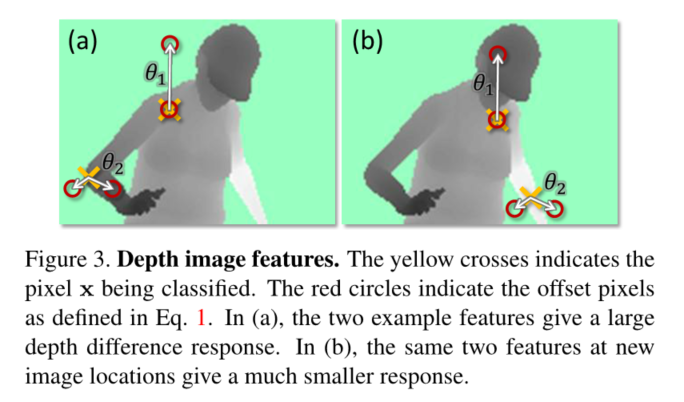
\includegraphics[width=0.45\linewidth]{figures/shotton2013real_features.png}
   \caption{\textbf{Shotton's Random Forest} \cite{shotton2013real}}
   \label{fig:shotton2013real_features}
\end{figure}
\end{enumerate}

% =============================================
Predicting Depth
% =============================================
Segmenting in 3D + time~\cite{hickson2014efficient}:
\blockquote{Our approach relies on the following observation: If the
scene consists only of convex objects, then every depth discontinuity
corresponds to an object boundary. This observation
was motivated by a study on primates [ref] which concluded
that depth and color perception are handled by separate
channels in our nervous system that function quite distinctly.
Obviously the world does not consist only of convex
objects, but nevertheless we have found this observation to
have great practical utility in everyday scenes. }

Eigen and Fergus~\cite{eigen2014predicting} predicts depth with CNNs.

% ====================
\section{Early Tracking}
% ====================
Tracking pre-2005ish.

CONDENSATION—Conditional Density Propagation for Visual Tracking: "The problem of tracking curves in dense visual clutter is challenging. Kalman filtering is inadequate because it is based on Gaussian densities which, being unimodal, cannot represent simultaneous alternative hypotheses. The CONDENSATION algorithm uses ``factored sampling'', previously applied to the interpretation of static images, in which the probability distribution of possible interpretations is represented by a randomly generated set. CONDENSATION uses learned dynamical models, together with visual observations, to propagate the random set over time. The result is highly robust tracking of agile motion. Notwithstanding the use of stochastic methods, the algorithm runs in near real-time."

http://www.cse.psu.edu/~rcollins/CollinsVLPR2012Lecture.pdf
http://www.cse.psu.edu/~rcollins/CollinsVLPR2009Lecture.pdf

% ====================
\section{Pedestrian Detection}
% ====================

Benson \etal~\cite{benenson2014ten}: 10 year review paper, starting to use optical flow

Object detection of a known object category is a well-studied problem. 
Benenson \etal~\cite{benenson2014ten} show four paradigms have emerged competitive: variants of Viola and Jones~\cite{viola2005detecting}, histograms of oriented gradients (HOG) classified by linear support vector machines (SVM) \cite{dalal2005histograms}, the deformable parts model (DPM)~\cite{felzenszwalb2010object} and convolutional neural networks.

% ====================
\section{Object Detection}
% ====================

Bjorn Ommer \cite{yarlagadda2014beyond, antic2014learning, eigenstetter2014randomized, monroy2012beyond} gave a talk at UBC: find 1000 random parts; group parts by their detection responses' spatial proximity in training data instances, then use those groups as positive examples for a part.

Ommer's ECCV 12 paper \cite{monroy2012beyond}:
\blockquote{we propose an approach for learning object models for detection
while, simultaneously, learning to segregate objects from clutter
and extracting their overall shape. For this purpose, we exclusively use
bounding-box annotated training data. The approach groups fragmented
object regions using the Multiple Instance Learning (MIL) framework to
obtain a meaningful representation of object shape which, at the same
time, crops away distracting background clutter to improve the appearance
representation.}

% ====================
\section{Object Proposals}
% ====================
Object proposals deal with finding interesting parts of an image.


Zitnick and Dollar's \cite{zitnick2014edge} Object Proposals from Edge Detections:
\blockquote{the number of contours that are wholly contained in a bounding box is indicative of the likelihood of the box containing an object. We propose a simple box objectness score that
measures the number of edges that exist in the box minus those that
are members of contours that overlap the box’s boundary. Using efficient
data structures, millions of candidate boxes can be evaluated in a fraction
of a second, returning a ranked set of a few thousand top-scoring proposals.
Using standard metrics, we show results that are significantly more
accurate than the current state-of-the-art while being faster to compute.}

\cite{zitnick2014edge} has a good overview of the field, as with Dollar's Nov 18th blogpost.

Uses Dollar's work on edge detection \cite{dollar2014fast}

% ====================
\section{Tracklet Proposals}
% ====================
Tracklet proposals deal with finding interesting tubes of the video

% ====================
\section{Edge Detection}
% ====================
Dollar's work on edge detection \cite{dollar2014fast}: uses random forests for structured prediction. Given 32x32 image patch, determine if each pixel in the centre 16x16 image patch belongs to an edge. Features: Piotr's integrated channel features, at each pixel and "pairwise difference features". Chug in Structured Random Forest. Achieves state of art with sharpening and multi-scale detection, running in real-time.

Idea: Dollar's work on RGBD Time series, with before and after frames.

On depth: Gupta's work outperforms Piotr's.




% ====================
\section{Thermal Images}
% ====================
Gade and Moeslund~\cite{gade2014thermal} give a good
overview of using thermal cameras. 
Teutsch \etal~\cite{teutsch2014low} also notes detection is a fundamentally different problem in thermal videos and thoroughly experiments with different feature sets for thermal object detection. 
A trend unique to thermal object detectors is the inclusion of a pre-processing step to find candidate regions of interest based on intensity, from which object detectors can then be used to classify the region.
Many object detectors in thermal images use shape-based features, often derived
from silhouettes identified by applying a threshold to intensity values.
Most thermal object detection focus on humans.

% ====================
\section{Understanding Natural Images}
% ====================
Lenc and Vedaldi~\cite{lenc2014understanding}: Understanding image representations by measuring their equivariance and equivalence

% ====================
\section{Techniques}
% ====================
\begin{enumerate}
\item Structured SVMs: vedaldi2014structuredsvm
\item Multi-resolution \cite{park2010multiresolution}: for finite resolution cameras, scale variance is needed.
\end{enumerate}

\textbf{FABMAP}:
Bag of words,  descriptor, vector quantization into a visual word, Chow-liu trees for bayesian probability

% ====================
\section{Machine Learning}
% ====================
Gaussian Processes Bible (with matlab toolbox) \cite{rasmussen2006gaussian}


% =============================================
\section{Pedestrian Path Planning}
% =============================================
ETH overhead dataset \cite{pellegrini2009you}

% ====================
% ===================================================
\chapter{Literature - Individual Paper Reviews}
% ===================================================
% ====================

If it's here, it's somewhat interesting.
% ====================
\section{Papers With Good Content}
% ====================
Zitnick and Dollar's Object Proposals from Edges \cite{zitnick2014edge}. Insanely fast and state of art.

Shotton's Random Forests \cite{shotton2013real}: Quality procedures (high quality training data), solves problem.



% ====================
\section{Papers Written Well}
% ====================
Anything by Piotr \cite{dollar2014fast}.

% --------------------
\subsection{Gao \etal~\cite{gao2014transfer}: Transfer Learning Based Visual Tracking
with Gaussian Processes Regression}
% --------------------
\paragraph{Summary} Another online tracking method. I haven't read into the technique yet.
\paragraph{Clarity} Quite clear. 
\paragraph{Method} Very legitamate, compares against top 3 benchmarks circa 2014.
\paragraph{Comments} They reference an astounding number of tracking papers. It seems sort of incremental and probably won't get cited. Why are people solving this problem? Who needs model-free online tracking?
